%% LaTeX2e class for student theses
%% sections/content.tex
%% 
%% Karlsruhe Institute of Technology
%% Institute for Program Structures and Data Organization
%% Chair for Software Design and Quality (SDQ)
%%
%% Dr.-Ing. Erik Burger
%% burger@kit.edu
%%
%% Version 1.3.3, 2018-04-17

\chapter{Visualization concept}
\label{ch:concept}

In the previous chapter we described how the interviews with the patent experts shaped our understanding of the patent landscaping task.
The knowledge gained in the process combined with the ideas gained from state-of-the-art approaches allowed us to develop a concept for the visualization.
In this chapter, we first outline the visualization concept in its final state.
We then cover the decisions that led to this stage.
Lastly, a brief summary of the data processing steps needed to produce document representations is given.
In the next chapter (\autoref{ch:implementation}), we present the separate components of the user interface of the visualization and of the data processing pipeline in their implemented form and discuss them in detail.


\section{Outline}
\label{sec:outline_visualization_concept}

In this work, we deal with semantic exploration of documents.
This refers to, on the one hand, the challenge of displaying high-dimensional \textit{semantic representations} of documents visually.
On the other hand, we support \textit{semantic interactions}, which means that the display adapts to the intentions of the user with regard to information density and level of detail.
These two topics are reflected in our concept.

A simplified representation of the visualization layout can be seen in \autoref{fig:schematic}.
The user interface consists of four interconnected parts: scatter plot, histogram, detail view and sunburst including breadcrumbs.

\textit{The scatter plot} is the main area of the visualization where each patent document is represented as a point.
Visualization space within the scatter plot is, effectively, the high-dimensional semantic space reduced to two dimensions. 
The user can navigate this space by panning and zooming (see \autoref{subsubsec:panning_and_zooming} for details on panning and zooming).
Each document is labeled by its relevant key terms which are extracted as described in \autoref{subsec:term_extraction}.
To keep the point labels readable, a heuristic is applied for optimal text density depending on the number of points within view and the zoom factor (see \autoref{subsubsec:points} ``Zooming'' for details).
Additionally, points and labels increase in size slightly to support the feeling of ``moving into'' the data.
Hovering over a patent makes its family connections, forward and backward citations to become visible as lines of different color and stroke type.

The documents are grouped into clusters that are characterized by a list of key terms.
The three most relevant key terms per cluster are always visible, and a full list of top 15 key terms is shown on demand when the user hovers over the cluster label.
Moreover, additional context for every single-word key term is provided by a list of words which are semantically similar to the term and occur often within the cluster.
We call those \textit{augmenting terms} and describe how they are generated in \autoref{subsec:hierarchical_clustering}.

There are three sizes of clusters produced by a hierarchical clustering algorithm.
As the user zooms into the scatter plot, large clusters are first substituted by medium-sized clusters and then by small ones.
This is an embodiment of the semantic zooming (see \autoref{subsubsec:semantic_zooming} for details on semantic zooming).

The histogram and sunburst views present metadata attributes from the dataset in an aggregated form. 
They enable filtering of the the data points within the scatter plot by brushing and linking (see \autoref{subsubsec:brushing_and_linking} for details on brushing and linking).
When filtering happens, a subset of the points in the scatter plot becomes grayed out, so that the user can focus their attention on the remaining documents.

\textit{The histogram} shows the temporal dynamics of patent activity represented by the number of patent applications per year.
A user can select a time interval by brushing .
A corresponding filter is then applied to the data.

\textit{The sunburst} is essentially a stacked pie chart.
It shows the distribution of patents across a given set of metadata attributes in the form of a hierarchy.
Patent assignee, country and \gls{ipc} classes can be used as levels for the sunburst hierarchy by themselves or in combination with each other.
The user can navigate back and forth between the sunburst hierarchy levels.
If one sector in the sunburst is clicked, it becomes the current root node and its children occupy the whole circle.
Then, with a click in the middle of the sunburst the user can go one hierarchy level up.
Moreover, colors of points in the scatter plot correspond to colors of sunburst sectors in their current state.
Pie-chart-shaped glyphs appear in place of points where there are multiple values per document, for example, multiple assignees.

The sunburst is complemented by \textit{breadcrumbs} analogous to the ones seen in website navigation.
They show the currently selected sunburst node and its predecessors.
After the breadcrumb path the percentage of all documents that correspond to the currently selected sunburst node is displayed.

\textit{The detail view} offers the possibility to study one patent document thoroughly in accordance with the principle of details-on-demand (see \autoref{subsubsec:visual_information_seeking_mantra} for details-on-demand).
The details for a patent become visible in the detail view when the patent is selected by clicking or hovered over.

All views are coordinated through user interactions, which fall into tree groups: selection, highlighting and resetting the current selection.
Those are implemented in a consistent way across all views: hovering with a mouse causes a highlighting of an object/group which is a preview of the selection, clicking means selecting an object/group and clicking on the background of a view resets the selection.
We apply the visual information seeking mantra (described in \autoref{subsubsec:visual_information_seeking_mantra}) to allow efficient exploration of the data.

\begin{figure}[!]
\centering
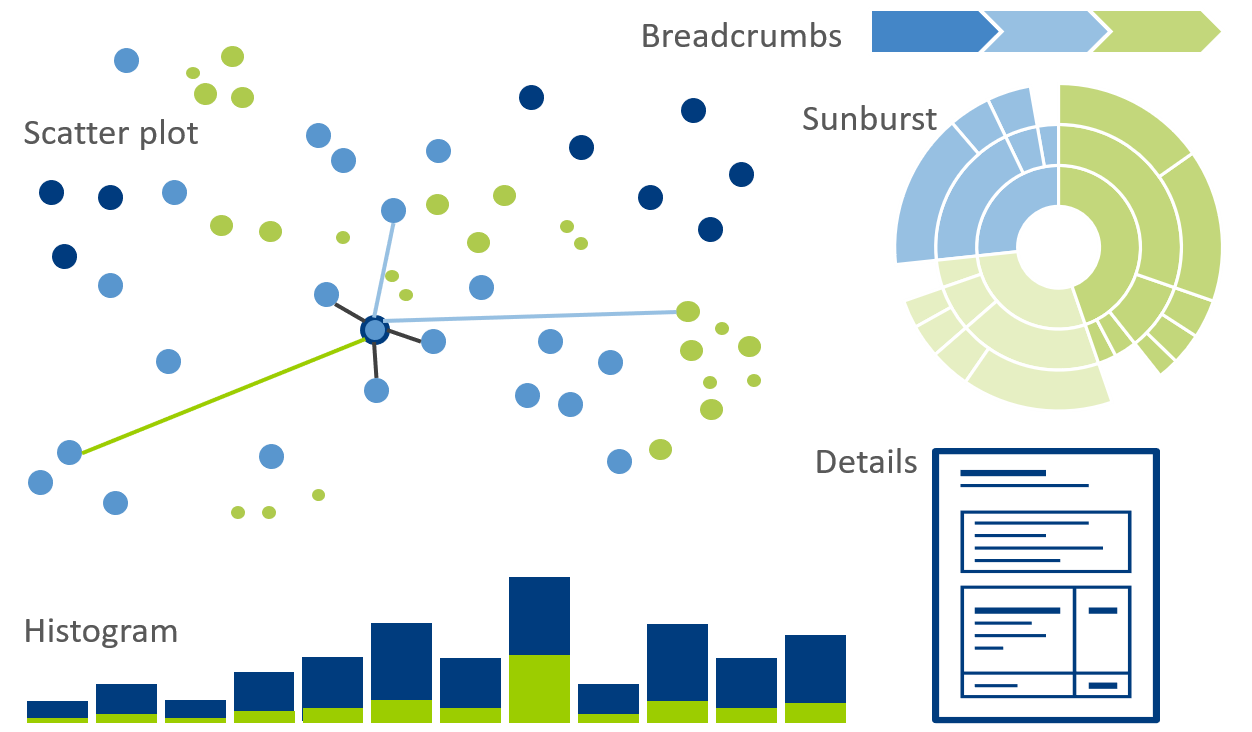
\includegraphics[width=\textwidth]{img/schematic}
\caption{A schematic representation of the visualization layout.}
\label{fig:schematic}
\end{figure}

\section{Ideation}
\label{sec:ideation}

In this section we justify the decisions that led to the creation of the visualization concept.
We then discuss the first iteration of the concept and the changes it went through during the development.

\subsection{Dimensionality of the visualization space}
\label{subsec:dimensionality_of_visualization_space}

The dimensionality of the embeddings that we intend to visualize is much too high to be plotted as it is.
A lower-dimensional presentation of the data must first be obtained via a dimension reduction technique. 
For that, a choice between 2D- and 3D-representation has to be made.
The latter provides an advantage in the sense that one additional dimension of the data can be displayed.
However, this gain comes with trade-offs with regard to usability.

Nielsen \cite{Nielsen1998} discourages using 3D for user interfaces.
He argues that while navigation in a 3D space looks impressive for an observer, it requires more cognitive resources from the user.
First, current interaction techniques are not specifically adapted for a 3D space and are cumbersome.
Second, even if the user successfully masters the controls, they still have to pay extra attention to navigating the 3D view in addition to navigating the information space.
The perspective itself introduces some usability problems. 
For example, remote objects are often hidden by nearby objects or are too small to be readable.
Additionally, it might be difficult to estimate the exact depth of an object or the distance between objects.

The plausibility of this line of reasoning has to be tested empirically.
Westerman et al. \cite{Westerman2000}, Banchs \cite{Banchs2014} and Fabrikant \cite{Fabrikant2007} performed comparison studies of 2D vs. 3D with regard to information retrieval tasks. 

Westerman et al. evaluated searching for objects in semantic spaces with multiple options for the amount of variance explained by all dimensions together.
They found that performance was generally poorer in three-dimensional condition with comparable amount of variance to a two-dimensional condition.
Moreover, they suggest that three-dimensional interfaces ``incur greater cognitive costs because of the demands of a more complex semantic mapping, i.e. maintaining a more complex mental model of the information space''.

In works of both Banchs and Fabrikant, 3D interfaces received positive feedback and were the participants' preferred representation.
In Banchs' study, the participants reported that the 3D platform allowed faster search, when in fact task completion times were lower for the 2D platform.
Notably, a higher percentage of tasks was accomplished successfully using a 3D platform.
Nevertheless, Banchs' conclusions match Nielsen's reasoning, namely that 2D interfaces are currently still more familiar to users.
Banchs highlights the performance of the visualization as one of the significant limitations, which was also mentioned by the participants.
This limitation also applies to our work, since our goal is to enable exploration of thousands of documents.

A notable exception from mentioned negative aspects constitute applications with entertainment purposes or for rendering physical objects in their solid form, where using 3D is encouraged \cite{Nielsen1998}.
Moreover, all above-mentioned arguments only apply assuming a pseudo-3D representation on a conventional two-dimensional computer screen.
A \gls{vr} application would define its own interaction techniques that feel natural for a 3D space.
Immersive data visualization in such environment using a \gls{vr} headset has been researched, for example in \cite{djorgovski2018immersive} and \cite{Hadjar2018}. 
Moreover, using a \gls{vr} environment implies a technology stack that is better adapted to displaying complex geometry, for example large point clouds.
Unfortunately, the advantages of a ``true 3D'' approach are not utilizable on a standard desktop workstation without extra hardware.

Ultimately, gaining one additional spacial dimension for representation is not worth the increased inconvenience of navigating the information space.
Therefore, we decided upon a 2D representation for our prototype.

\subsection{Choice of a suitable visualization metaphor for hierarchical data}

Most of the patent metadata attributes are of relatively common data types like date, string or list of strings.
But there is one attribute with an uncommon type and that is the \gls{ipc} class (described in \autoref{subsubsec:ipc_classification}), or more specifically, a list of \gls{ipc} classes.
\gls{ipc} classes are hierarchical in nature, which necessitates a suitable visual metaphor.

The \textit{treemap} as shown in \autoref{fig:treemap} is a space-filling type of diagram that was proposed by Shneiderman \cite{Shneiderman1992} and has often been used to visualize hierarchical data.
It uses nested shapes, usually rectangles, to represent the parent-child relationship.
A parent rectangle's space is divided into child rectangles along an axis that changes with each nesting level.
Size and color of rectangles represent various attributes of hierarchy nodes.
In an interactive version of a treemap, the user can select a node to examine its children in detail.
The available space is then redistributed to a subset of the hierarchy with the chosen node as its top.

\begin{figure}[!]
\centering
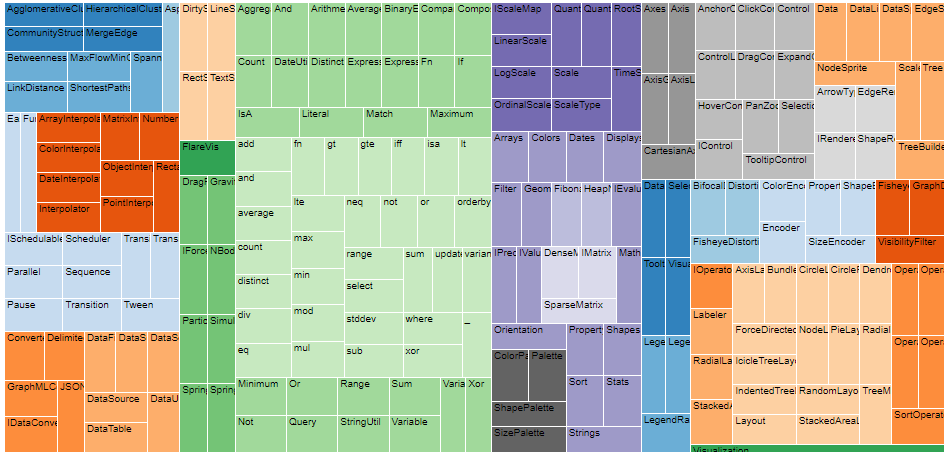
\includegraphics[width=0.7\textwidth]{img/treemap}
\caption{Treemap visualization of the class structure in a programming library Flare. Source: \cite{Takayuki2016}}
\label{fig:treemap}
\end{figure}

The \textit{sunburst} type of diagram was inspired by the treemap. 
It utilizes a radial layout in which child nodes are not contained in the parent nodes, but expand outwards from the circle center.
Size (angle) and color of the radial sectors can, just as with a treemap, represent chosen attributes of nodes in a hierarchy.
One can also navigate within the hierarchy by choosing a node to serve as a starting point in the center.

\cite{Stasko2000} evaluated treemap and sunburst in their study.
Their conclusion was that the sunburst ``more frequently aided task performance, both in correctness and in time, particularly so for larger hierarchies. The explicit portrayal of structure appeared to be a primary contributor to this benefit.''
Supported by this finding, we initially chose to use a sunburst for a fairly large hierarchy that is the \gls{ipc} classification.
Later, an idea emerged that the attributes represented by sunburst do not necessarily have to be of a hierarchical nature.
It is possible to ``stack'' multiple categorical attributes, for example country and assignee, to produce subgroups/child nodes which are represented in a sunburst.
Moreover, it is also possible to combine categorical and hierarchical attributes to show, for example, a distribution of \gls{ipc} classes per country.
In our visualization concept, we evaluate the feasibility of using metadata attributes of various types in a sunburst diagram.

\subsection{Initial concept and its evolution}
\label{subsec:initial_concept}

The initial concept was inspired by a demonstration of coordinated views showing mock data by \cite{Johnson2018}.
This demonstration implemented brushing and linking (see \autoref{subsubsec:brushing_and_linking} for more on brushing and linking).
The demonstration consists of a scatter plot on the left, a histogram on the right and an additional representation of a time axis at the bottom (see \autoref{fig:idea}).

\begin{figure}[!]
\centering
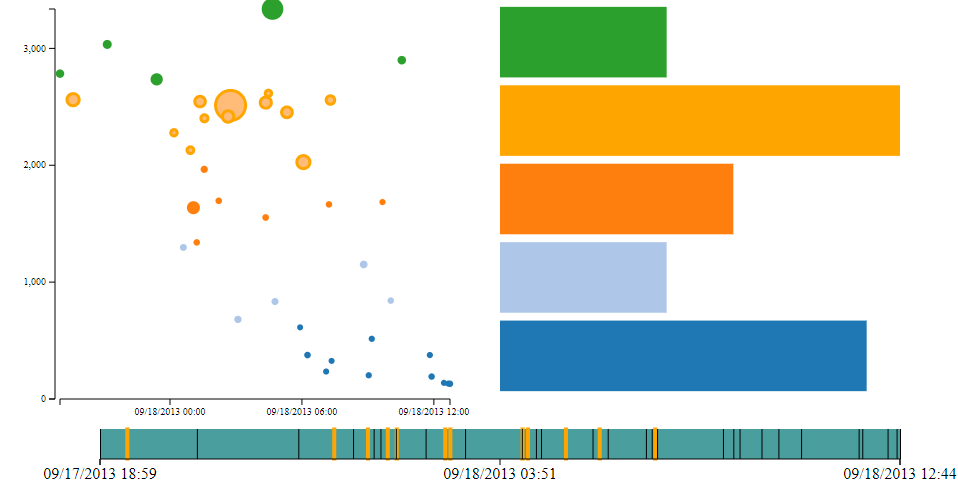
\includegraphics[width=\textwidth]{img/idea}
\caption{Demonstration of coordinated views that served as an inspiration for our concept. Image source and demo: \cite{Johnson2018}}
\label{fig:idea}
\end{figure}

The Y-axis of the scatter plot corresponds to a numerical dimension in the mock dataset, while the X-axis represents timestamps of data points.
The histogram splits the values of the numerical dimension into five bins.
The element at the bottom of the demo is essentially a \textit{rug plot}, i. e. it denotes the X-positions of data points by tick marks that look similar to tassels on a rug.
A classic example of a rug plot can be seen in \autoref{fig:rug_plot}.

\begin{figure}[!]
\centering
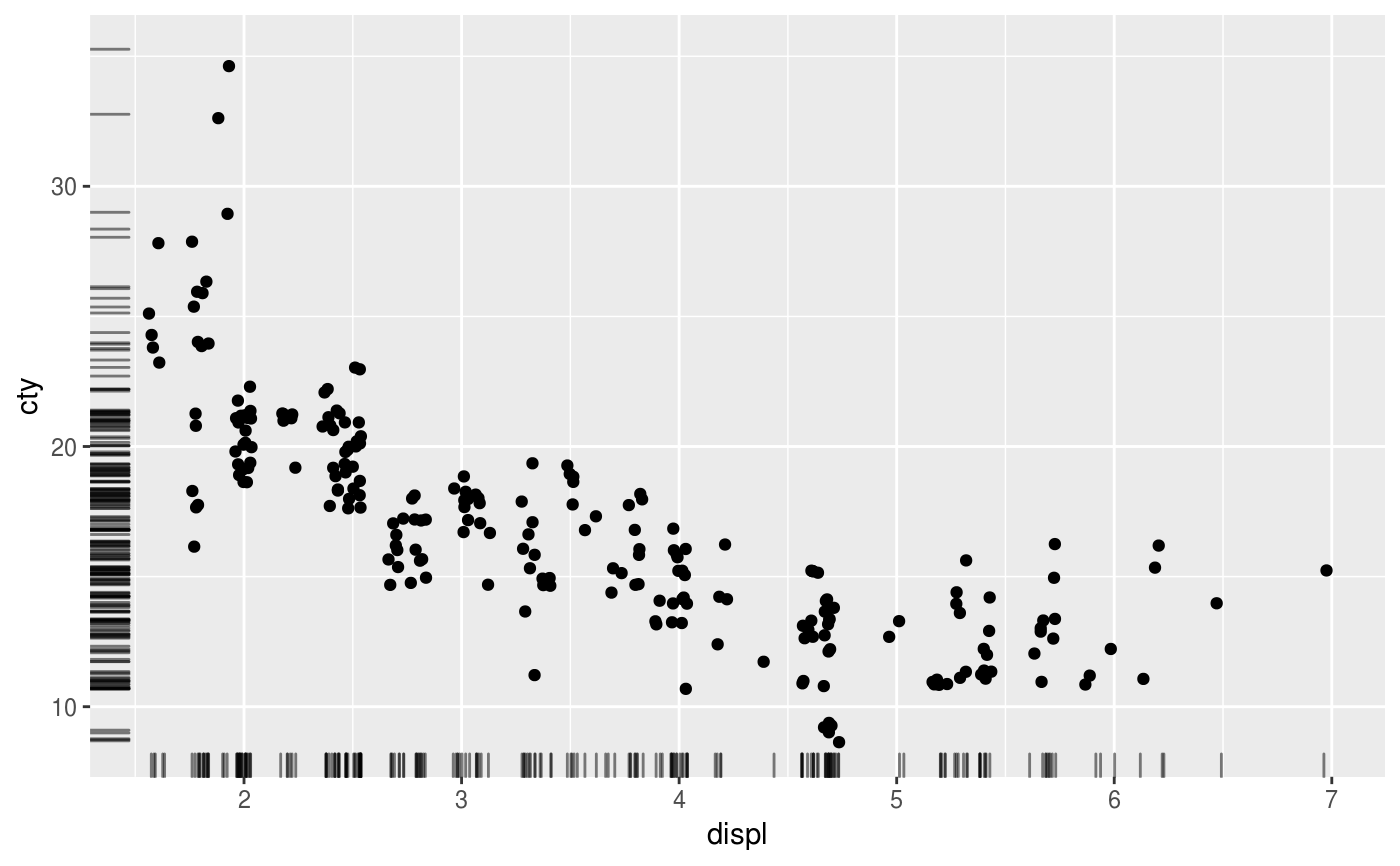
\includegraphics[width=\textwidth]{img/rug_plot}
\caption{A scatter plot is augmented with a rug plot. The rug plot shows distribution of the data points with regard to X and Y coordinates. Image source: \cite{rug}}
\label{fig:rug_plot}
\end{figure}

Rug plots are used to illustrate the distribution of a variable along the axes, in this case the time axis.
Usually, a rug plot is drawn as a part of the original plot (scatter plot, line plot, histogram, etc.), but in this instance it has been separated from the corresponding scatter plot.
The main purpose of the element is to enable selection of the data by brushing and linking, which is why we and the author refer to it as the \textit{brush element}.
The histogram values are recomputed in accordance with the updated selection.
Moreover, when the mouse is hovering over the histogram bins, corresponding data points are highlighted both in the scatter plot and in the brush element.

The first iteration of our visualization concept  (see \autoref{fig:sketch}) was built on ideas borrowed from the above-mentioned demonstration by \cite{Johnson2018}.

\begin{sidewaysfigure}
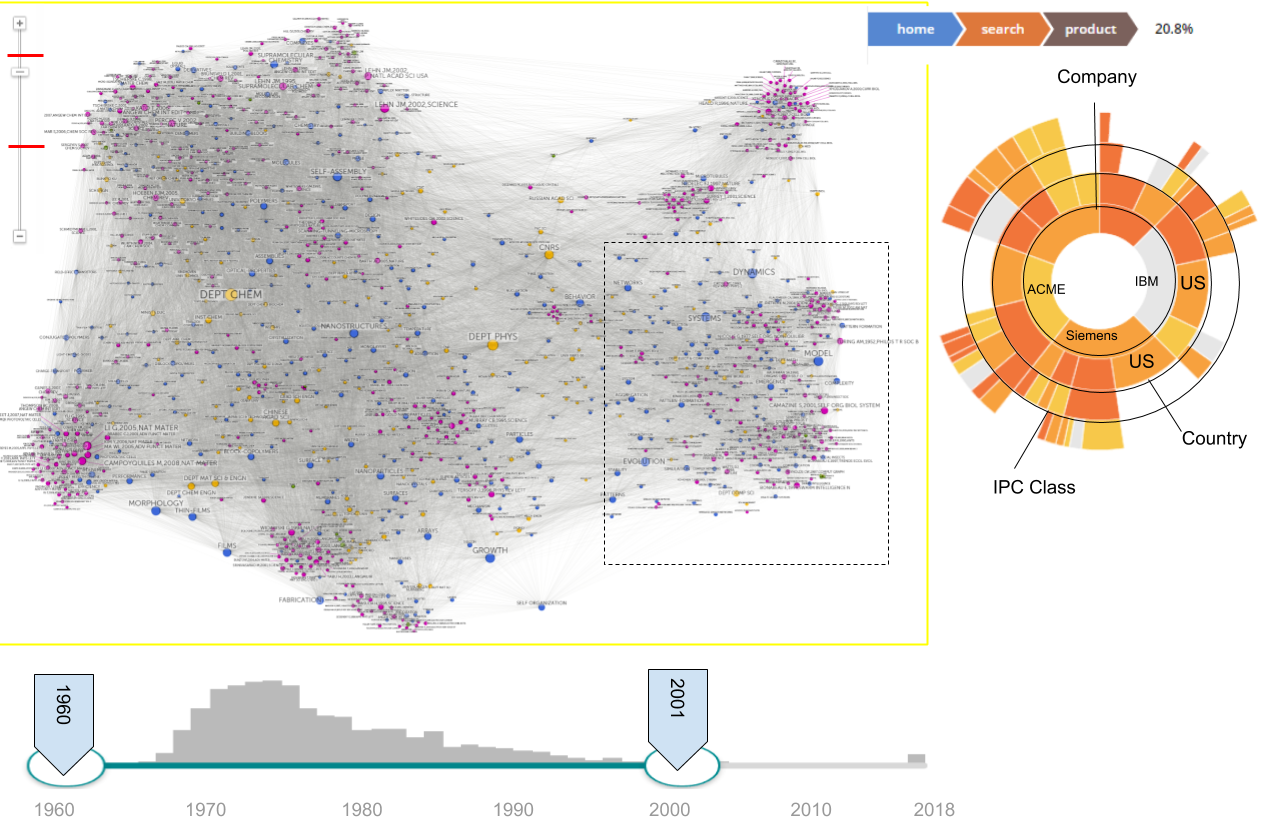
\includegraphics[width=\textwidth]{img/Visualization_mockup}
\caption{The first iteration of the visualization concept. Source of the graph picture: \cite{Latour2012}, source of the sunburst picture: \cite{Ribecca2019}.}
\label{fig:sketch}
\end{sidewaysfigure}

Firstly, it was the idea of a main area that contains data points and is influenced by controls on the edge of the display.
Displaying distribution of patent applications over time and the ability to select a time interval we consider especially useful for the patent landscaping use case.
Therefore, we decided to implement the same linking and brushing functionality, yet considering the size of the data, a histogram with yearly bins was judged more fitting to show the distribution over time.

Secondly, inspired by the ideas from \cite{Johnson2018} and \cite{Wittenburg2015}, our UI concept was designed to show a distribution of the dimensions of the data.
In our case those attributes are mostly categorical, and \gls{ipc} classes are also hierarchical in nature.
The wish to display multiple dimensions of the metadata resulted in our choice of a sunburst chart in the place of a histogram in the original demonstration.
This decision was partly motivated by Wittenburg et al. \cite{Wittenburg2015}, who make extensive use of metadata in their faceted visualization (see \autoref{fig:wittenburg}).
They show the assignee, country and application year as a vertical stack of blocks where the width of a block corresponds to the number of patents with the corresponding attribute value. 
Unfortunately, their approach results in a cluttered view and therefore lacks visual scalability.
We address the scalability problem via interactivity, i. e. through the fact that it is possible to change levels of a sunburst chart 1) through navigating up and down the hierarchy of attributes and 2) by choice of different sets of metadata attributes to be charted.
For more details on our implementation of the sunburst chart see \autoref{subsec:sunburst_and_breadcrumbs}.

The main area of our visualization was initially conceived as a fully connected graph.
Similarities between each pair of documents were supposed to correspond to the attraction forces in the force-directed graph layout.
When a part of the dataset would be eliminated through filtering, the corresponding graph nodes would disappear and the whole layout would rearrange itself.
Effectively, the process would amount to computing and then dynamically updating a \gls{tsne} representation of the dataset. 
An interactive demonstration of such a layout is presented in \cite{Strayer2018}.
While it would certainly be of value to cluster subsets of the data dynamically depending on the selection, performance considerations outweigh the benefits.
Therefore, a scatter plot with static positions of data points was chosen as a viable alternative.

Initially, the concept included no standalone detail view.
Instead, the idea was to display some tooltip elements directly above the currently chosen patent and above patents related to it.
Type and amount of the information presented in the tooltips were supposed to change depending on current selection and zoom level according to the principle of \textit{semantic zooming}.
Upon further consideration it became clear that such tooltips would cover a significant portion of the scatter plot and would therefore render it unusable.
The decision was made to place the detailed patent information to the available space in the lower-right corner.

The zoom control in the upper-left corner is an idea borrowed from various interactive map interfaces.
The red markings were supposed to show boundaries between different detail levels of hierarchical clustering.
Ultimately, we implemented different visual indications that sufficiently support the feeling of ``moving into'' the landscape and back, so this part of the initial concept was omitted.
Other elements were utilized in the prototype without changing much.

\section{Data processing}
\label{sec:pipeline}

Before a dataset can be displayed in a visualization, it has to be processed in a preparatory step.
\autoref{fig:pipeline_single} and \autoref{fig:pipeline_all} present an overview of the processing pipeline which is necessary to produce data for the visualization.
In this section, we give a brief overview of the steps, which are covered in more detail in \autoref{sec:implementation_of_data_processing}.

\begin{figure}[!]
\centering
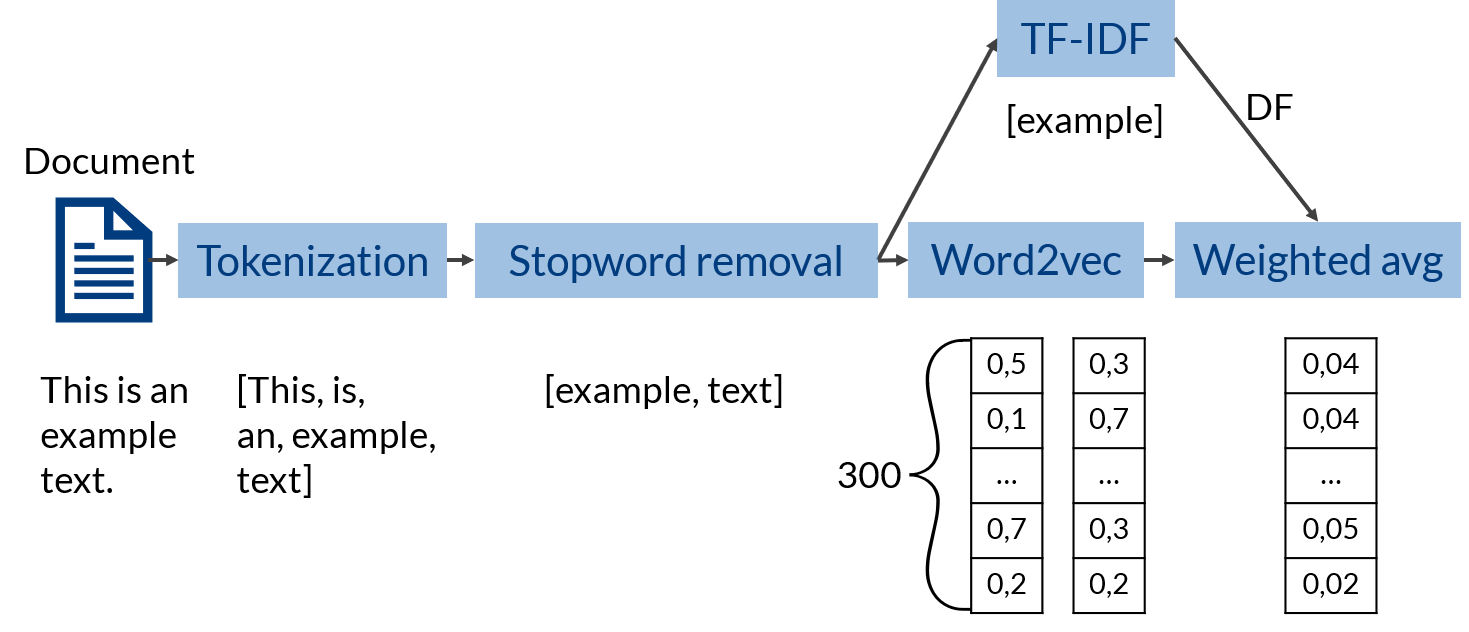
\includegraphics[width=0.9\textwidth]{img/pipeline_single}
\caption{Pipeline of processing steps for a single patent document}
\label{fig:pipeline_single}
\end{figure}

First, each patent needs to be processed individually (see \autoref{fig:pipeline_single}).
This starts with splitting the textual part into separate words and removing stopwords.
Stopwords include general grammar-related words such as ``is'', but also patent-specific vocabulary such as ``embodiment''.
Then, for each word a 300-dimensional embedding is retrieved from the word2vec model explained in more detail in \autoref{subsec:data_source}.
A vector representing the whole document is composed by aggregating the word vectors as a weighed average.
Each word is weighted with its IDF.
Our purpose is to make semantic similarities and differences tangible, but numerical document vectors do not provide an explanation of why any pair of documents are close or distant. 
Therefore, TF-IDF is also used to extract relevant key terms per patent.

\begin{figure}[!]
\centering
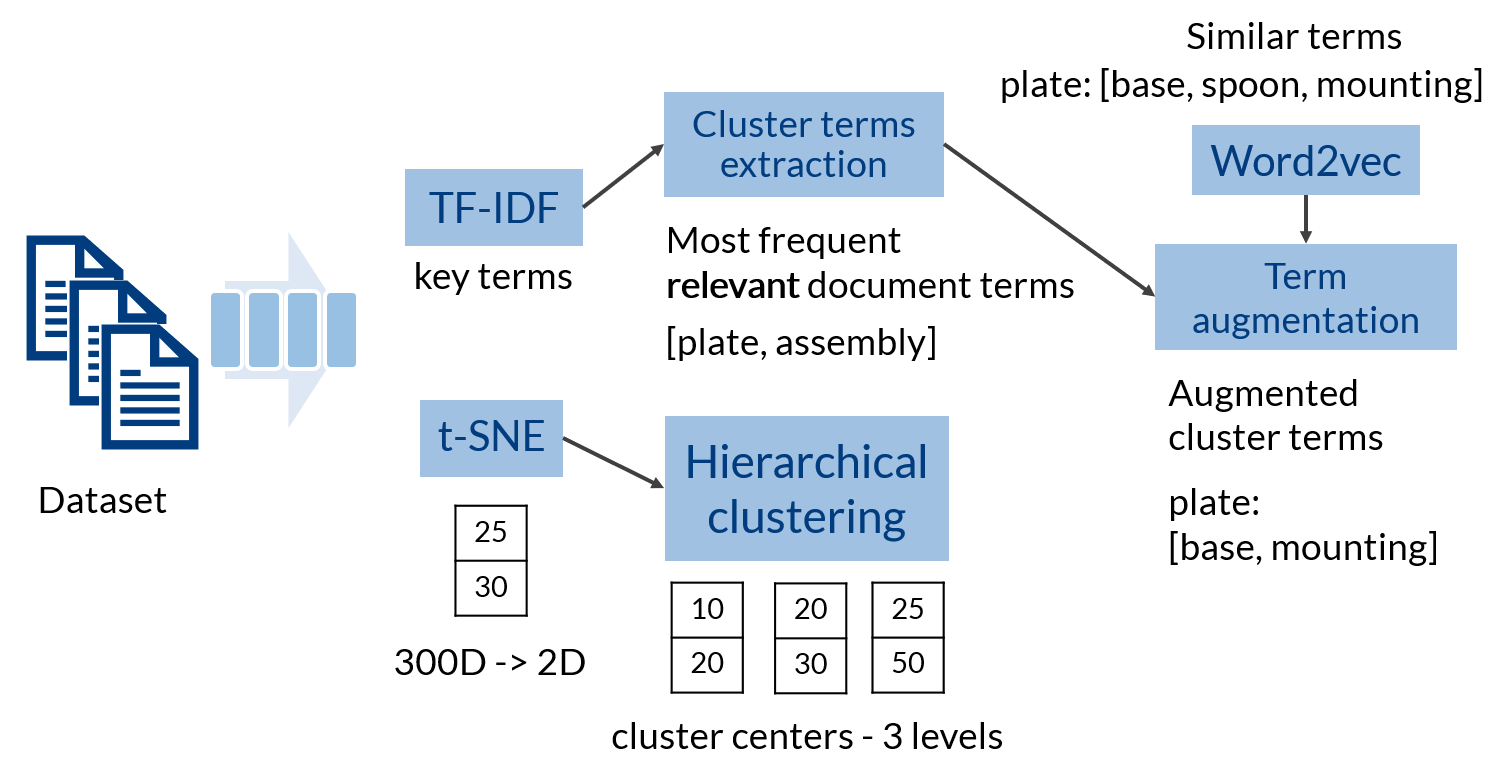
\includegraphics[width=0.9\textwidth]{img/pipeline_all}
\caption{Continuation of the pipeline after all individual patents have been processed}
\label{fig:pipeline_all}
\end{figure}

Second, after all document vectors and document key terms are computed, the processing on the dataset as a whole can begin (see \autoref{fig:pipeline_all}).
300-dimensional document vectors are reduced to two dimensions with \gls{tsne} to fit the visualization space.
This enables hierarchical clustering, which splits the dataset into a number of clusters on three detail levels, resulting in large, medium and small clusters.
It is crucial for user's understanding to know what common semantic characteristics the grouped patents share.
To cover that, we extract the key terms per cluster.
We take most relevant terms per document and count them across all patents within a cluster. 
The terms with most occurrences are assigned to the cluster to explain its thematic focus.

To aid the understanding of cluster key terms, for each single-word term we retrieve similar words from the above-mentioned word2vec model.
We then check whether those similar words occur in more than 10\% of the patents in the cluster.
If that is the case, the word is added to the list of augmenting terms for the given key term.
For example, if we try to augment the term \textit{plate}, the word2vec model might retrieve \textit{base, spoon, mounting} as similar words because they often appear in similar contexts with \textit{plate}.
Assuming the dataset is not about cutlery, \textit{spoon} does not appear in many patents, but \textit{base} and \textit{mounting} might. 
Therefore, \textit{base} and \textit{mounting} are the terms that provide context for the term \textit{plate} in the given cluster.

Herewith the processing of the textual part of the patent dataset is complete.
As for metadata, some of the attributes can be used in the visualization as is, while others require special processing (see \autoref{subsec:data_preprocessing} ``Parsing of metadata attributes'' and \autoref{subsec:hierarchies}).
We elaborate on the processing of both textual and metadata parts of a patent dataset in \autoref{sec:implementation_of_data_processing}.

